% TODO: 
% * fix organisation/organization
% * give lab access switches special treatment?
% * do we want to clearpage before \section's?
% * Phyical security!
% * centre vs center
% * clean up \\\\'s to look good and uniform
% * call our PT implementation a demo?
% * Run spellchecker
% * formatting for IP addresses? :/
% * replace "'S" with "'s"
% * branch -> learning centre
% * Gjøre guests større?
% * VLANs to VLAN's and so on
% * Make it clear that we are focusing on saving costs. Redundancy at the HQ for example is a luxury

\documentclass[a4paper,11pt,pdftex,english]{article} % change to norsk for Norwegian abstract and references

\usepackage{babel}
\usepackage{amsmath}
\usepackage{graphicx}
\usepackage[utf8]{inputenc}
\usepackage{epsfig}
\usepackage{graphicx}
\usepackage{palatino}
\renewcommand{\ttdefault}{lmtt}
\usepackage{enumerate}
\usepackage{mdwlist}
\usepackage{geometry}
%\usepackage{textcomp}
%\usepackage{type1cm}
\usepackage[table]{xcolor}
\usepackage{varioref}
\usepackage{url}
\usepackage[bookmarks=true, linkcolor=blue,
citecolor=blue,urlcolor=blue,colorli nks=true, breaklinks=true,
pagebackref=true, hyperindex=true,bookmarksopen=true]{hyperref}
\usepackage[shortlabels]{enumitem}
\newlist{arrowlist}{itemize}{1}
\setlist[arrowlist]{label=$\Rightarrow$}
\usepackage{minted}
\usepackage[strings]{underscore}
\usepackage{dirtytalk}

\graphicspath{ {./images/} } % make LaTeX look for images in the images folder


\frenchspacing

%% Block style paragrphs
\setlength\parskip{\medskipamount}
\setlength\parindent{0pt}

\makeatletter
\renewcommand{\topfraction}{.9}
\renewcommand{\bottomfraction}{.8}
\renewcommand{\textfraction}{.15}
\renewcommand{\floatpagefraction}{.66}
\renewcommand{\dbltopfraction}{.66}
\renewcommand{\dblfloatpagefraction}{.66}
\setcounter{topnumber}{9}
\setcounter{bottomnumber}{9}
\setcounter{totalnumber}{20}
\setcounter{dbltopnumber}{9}

\makeatother



\title{Charity Organization - "SikreNorge"}

% TODO: replace 923 with actual student number
\author{
  Job Nestor Bahner, 923\\
  Johannes Borgen, 923\\
  Abdisalan Hussein, 923\\
  Sam Roen, 923\\
  Thomas Løkkeborg, 923
}

\begin{document}

\maketitle

\begin{abstract}
  SikreNorge is a non-profit charity organization with locations all over Norway. In this report we will discuss how we would implement a network infrastructure for the organization.
\end{abstract}

\thispagestyle{empty}

\clearpage
\pagenumbering{roman}
\setcounter{page}{1}
\tableofcontents

\clearpage
\pagenumbering{arabic}

% BEGINNING OF CONTENT

\section{Business case}

SikreNorge is a non-profit charity organization that provides information security services to businesses and institutions in Norway. The organization seeks to secure Norway by helping those who would not otherwise have the means to prioritize security.
\\
\\
Financially SikreNorge relies on donations, government subsidies, and income from their web-shop. Businesses who donate are encouraged to publicise their contribution to show that they support the organization's mission. This way both the contributing businesses and SikreNorge get good PR. Government subsidies are given with the intention and expectation that the organization will use these means to support local public and private institutions with information security tasks.
\\
\\
The organization is reliant on local expertise in each county in the form of volunteers and hired professionals. Volunteers are expected and encouraged to gain security competence through the experts. Good candidates for volunteers are students doing technical studies. Where possible the organization will make agreements with local universities teaching information technology courses to encourage students to volunteer. The organization is also open to volunteer work as part of theses and course projects. Volunteers of the organization do work in exchange for practical information security experience. Both volunteers and hired professionals are expected to sign strict non-disclosure agreements regarding their work with businesses and institutions.

\subsection{Locations}

SikreNorge will establish learning centers in each of Norway's 19 counties. The headquarter lies in Oslo.

% TODO note that the number of counties is changing
Learning centers are meant as a hub for all the organizations activities in the county. The centers have offices for local management and hired professionals. They also contain network sandbox areas for practicing network security, classrooms for security courses, lecture halls for seminars and general storage space. In addition to activities held at the centers, the organization can send consultants into the field to do evaluation or configuration on-site. Consultants are a mix of local hired professionals, volunteers and staff.
\\
\\
The organization's headquarter provides the same services as learning centers, but also does the heavy lifting in terms of information technology services and infrastructure. The website, E-mail, management applications, and all the large equipment to which one can connect from another center for data resources are examples of services that are hosted here.

\subsection{Services}

The organization includes a wide range of services, and the network must be set up to support these. Following is a brief discussion of key services, along with some infrastructure concerns.

% TODO more services?

\subsubsection{On-site company consultation}

Volunteers, hired professionals and staff  can be sent out to do consulting on-site at businesses or institutions. Access to the organizations internal services might be required during consultation, so the consultants should be able to reach them from on-site. Confidential information might be sent and received during this communication, so the technology chosen for this should focus on security.

\subsubsection{Teaching at learning centre}

Businesses and institutions may visit a learning centre to take courses or to receive guidance. During this stay they will naturally want internet connectivity. In addition, access to some internal services might be needed for training purposes. A visitors access rights should be restricted as much as possible.

\subsubsection{Network security laboratory}

Each learning centre has a laboratory where visitors can explore hardware and software to learn about vulnerabilities and best practises. Labs are meant to be a sandbox area for learning about information security, so they should be separated from the rest of the distribution system in such a way that experiments from the lab cannot interfere with the rest of the learning centers operations.

% TODO "separated from the rest of the distribution system" - currently this is not done

\subsubsection{Public website}

SikreNorge's website includes information about the organizations offerings, online courses and a web-shop. Some of the website's information and courses might build upon internal services, so the infrastructure should support communication to allow this. The web-shop will sell T-shirts, coffee mugs, posters and more to further information security awareness and good practise. The shop allows buyers to register accounts for easy shopping.

\subsubsection{Management website}

The organization uses a website separate to the public website to manage internal logistics. Registered staff, businesses, institutions and overview of future work are examples of information that can be found here.

% TODO: refer do the bave and below sections in the ict implementation discussion

\clearpage

\section{Security Policy}

% NOTE BY THOMAS: This list was slightly changed from the one in docs, as LaTeX struggles with lists deeper than 4 levels :p

\subsection{Statement of policy}

\begin{enumerate}
  \item Scope and applicability
  \begin{enumerate}
    \item Our organization
      \begin{enumerate}
        \item Every member is expected to know the content of our policy and comply. Ignorance is equal to non compliance.
      \end{enumerate}
        \item Partners
      \begin{enumerate}
        \item To collaborate they are expected to know the content, whereas an equal understanding of security is key.
      \end{enumerate}
        \item Guests/Trainees
      \begin{enumerate}
        \item Should know key elements to ensure safe learning and usage when using our equipment. Coordinators should brief them before actual usage.
      \end{enumerate}
  \end{enumerate}
\end{enumerate}

\subsection{Definition of technology addressed}

\begin{enumerate}
  \item Use of Internet
  \begin{enumerate}   
    \item E-mail
    \item Browsing
  \end{enumerate}
  \item Use of organization equipment
  \begin{enumerate}
    \item Computers
    \item Servers
    \item Routers
    \item switches
  \end{enumerate}
  \item Use of partners or other non-organizational equipment
  \begin{enumerate}
    \item Personal equipment
    \item Tech brought by guest lecturers
  \end{enumerate}
  \item Use of telecommunications
  \begin{enumerate}
    \item Fax
    \item Phone
    \item VoIP
  \end{enumerate}
  \item Use of photocopy equipment
  \begin{enumerate}
    \item Hard copies
    \item Photographs 
    \item No personal documents: Passports etc.
  \end{enumerate}
\end{enumerate}

\subsection{Responsibilities}

\begin{enumerate}
  \item CISO 
  \begin{enumerate}
    \item Controls the overall structure of security and security management.
    \item Must adhere to security guidelines and practice consistently, as they are a possible single-point-of-failure in the security scheme.
    \item Must have It-Security background, in conjunction with management background.
  \end{enumerate}
  \item Branch office security managers
  \begin{enumerate}
     \item Manage security for their branch office.
     \item Report to CISO
  \end{enumerate}
  \item Employees
  \begin{enumerate}
    \item Be loyal to the organization's security guidelines.
    \item Understand Policy
    \item Validate understanding of policy
    \item Understand repercussions of policy insubordination
  \end{enumerate}
\end{enumerate}

\subsection{Authorized access}

\begin{enumerate}
  \item User access
  \begin{enumerate}
    \item Administration/management and other vital parts of the organizational systems are to be separated from normal users.
    \item Employees have a level of clearance, and access thereafter. 
    \item CISO have full access to systems.
    \item Employees with access to confidential classified information or higher must sign a non-disclosure agreement.
    \item Levels of classification on information:
    \begin{enumerate}
      \item Official - All can access.
      \item Confidential - Employees
      \item Restricted - Managers, CISO
      \item Secret - Executives
    \end{enumerate}
  \end{enumerate}
  \item Fair and responsible use
  \begin{enumerate}
    \item As a precaution, emails are to be treated critically.
    \begin{enumerate}
      \item Hyperlinks should not be clicked.
      \item Images not to be loaded before sender is verified.
      \item Autoload should remain off by default.
      \item Attachments not to be downloaded/viewed unless verified sender.
    \end{enumerate}
    \item Passwords should have a certain standard.
    \begin{enumerate}
      \item Not easy to crack.
      \item Least 10 characters.
      \item Non dictionary words or other easily identifiable words.
      \item Mix of characters (lower-, and uppercase), numbers and symbols.
      \item Separate from personal passwords.
      \item Password manager on organization equipment encouraged. Required for individuals with high clearance.
    \end{enumerate}
    \item VPN required off-site.
  \end{enumerate}
  \item Protection of privacy
  \begin{enumerate}
    \item Must adhere to GDPR regulations.
    \item Must also comply with regulations from Datatilsynet.
    \item Must comply with Norwegian and international laws
  \end{enumerate}
\end{enumerate}

\subsection{Prohibited usage of equipment}

\begin{enumerate}
  \item Disruptive use and misuse
  \begin{enumerate}
    \item No personal equipment in restricted areas.
    \item USB devices should only be issued by the organization
    \item Vital organizational equipment should not be brought off-site.
    \item Restricted equipment should not be used for not-intended purposes.
    \begin{enumerate}
      \item Web surfing
      \item Farming(Unless intended)
      \item Hosting(Unless intended)
      \item Packet sniffing(Wireshark, unless intended)
    \end{enumerate}
  \end{enumerate}
  \item Criminal use
  \item Offensive or harassing materials
  \item Copyrighted, licensed, or other intellectual property
\end{enumerate}

\subsection{Systems management}

\begin{enumerate}
  \item Management of stored materials
  \begin{enumerate}
    \item Authentication and authorisation should be managed by an AAA server and accounted.
    \item Classified data need to be encrypted on the hard drive and in transfer - Partner and organizational data protected by non-disclosure contracts.
    \item All organization equipment that have been used to store organisation or partner information must be disposed of in a safe manner.
    \item Hard drives must be destroyed by the organization itself.
    \item Printers must be in an enclosed network, and classified documents should only be printed on secure organization printers.
  \end{enumerate}
  \item Employer monitoring
  \begin{enumerate}
    \item Use of internet logged.
    \item Organizational equipment inventory checked regularly.
    \item Restricted area entry logged.
    \begin{enumerate}
      \item Physical - ID card entry log.
      \item Digital - Credentials log.
    \end{enumerate}
  \end{enumerate}
  \item Virus protection
  \begin{enumerate}
    \item Each branch need its own firewall.
    \item Organization computers and phones with internet connection need antivirus.
    \item Email etiquette, see Fair and responsible use( i ).
  \end{enumerate}
  \item Physical security
  \begin{enumerate}
    \item Limited access to restricted areas.
    \begin{enumerate}
      \item Must use ID-card to enter: Server rooms, Offices for high clearance individuals.
    \end{enumerate}
    \item Guest premises must be separated from working grounds and other vital instances.
  \end{enumerate}
  \item Encryption
  \begin{enumerate}
    \item Within the organization the use of asymmetric encryption with security level equal to SHA 3 or higher should be enforced.
  \end{enumerate}
\end{enumerate}

\subsection{Violation of policy}

\begin{enumerate}
  \item Procedures for reporting violations
  \begin{enumerate}
    \item As a security pushing organization, reporting violations of our policy is encouraged.
    \item To ensure this practice the report can be submitted anonymously.
  \end{enumerate}
    \item Penalties for violations
  \begin{enumerate}
    \item Minor voilations can result in revoked clearance or access.
    \item Serious violations:
    \begin{enumerate}
      \item Subject to dismissal.
      \item Legal action.
    \end{enumerate}
  \end{enumerate}
\end{enumerate}

\subsection{Policy review and modification}

\begin{enumerate}
  \item Scheduled review of policy modifications for modification
  \begin{enumerate}
    \item This organization will actively seek to be in the front of information security, to ensure we are able to offer our services with satisfaction. This policy is therefore an iterative peace of document which is subject to alteration if needed.
  \end{enumerate}
  \item Legal disclaimers
\end{enumerate}

\subsection{Limitations of liability}

\begin{enumerate}
  \item Statements of liability
  \begin{enumerate}
    \item This organization is not liable if an employee does not comply with our policy.
    \begin{enumerate}
      \item The organisation will assist in prosecution if necessary.
    \end{enumerate}
  \end{enumerate}
  \item Other disclaimers as needed
\end{enumerate}


\clearpage

\section{Risk assesment}

\textit{Following was copied from docs:}

One of the biggest risks is the theft, loss or unauthorized access of confidential data. Especially data that may be stored about partners and others we offer services to.
\\
\\
Since we rely on hired professionals and volunteers which must have some level of access to perform their work. A possible risk may be infiltration and espionage as well as theft of assets under the disguise of altruism.
\\
\\
Others may also try to gain physical unauthorized access to our and partner premises.
\\
\\
Our role in the public can make us a target for Distributed Denial of Service attacks (DDoS).
\\
\\
As everyone else we are at risk of human error and/or failure without mischievous or criminal intent. 
\\
\\
Power outage, natural disasters.

\clearpage

\section{ICT and Network Infrastructure}

% TOPICS TO DISCUSS, IN AN INITIAL ORDER:
%
% * include logical and physical view, and disucss briefly how to view the diagram. used in comming sections (?)
% * talk about WAN connection
% * Talk about subnets and VLANs and so on
% * talk about wireless and so on
% * talk about lab area
% * Branch specific stuff
%   * dhcp on the router
%   * firewall on the router
% * HQ specific stuff
%   * redundancy, loadbalancing (glbp)
%   * services area, redundancy there etc
%   * what goves over WAN
%   * "remote commuting" (if that's what it's called)

\textit{Short flavortext about what will be discussed}


\subsection{Diagrams}

\textit{Show logical and phyical views, and provide some discussion around them}


\begin{figure}[H]
\caption{Phyical view of the network (TEMPORARY)}
\centering
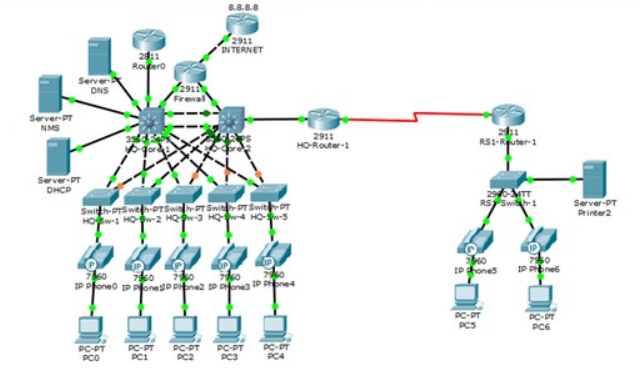
\includegraphics[width=\textwidth]{physicalviewtemp}
\label{physicalview}
\end{figure}

\subsection{WAN}

\textit{Discuss our WAN setup}

\subsection{Subnetting and VLANs}

When deciding how to do our subnets and VLAN's we decided to go for simplicity. We chose to subnet our private addresses from the 10.0.0.0/8 private address range, as it gave us plenty of space to the subnets up how we wanted. We dedicate the second octet to indicate what location the subnet belongs to, where the value 1 indicates the HQ, and a value above 1 indicates a branch site. For example: 10.1.x.x is a subnet the HQ, and 10.2.x.x is a subnet at the first learning centre and so on. This lets us create subnets that look very similar across locations, while letting a network engineer quickly see what location a particular IP address belongs to. We dedicate the third octet to indicate what VLAN the subnet belongs to, with the value of the octet being the same as the VLAN id. 10.1.10.x is a subnet for the management vlan of the HQ, and 10.10.60.x is a subnet for the printer VLAN of location nr 9. Combined with the fact that we reserve the first 10 hosts for static IP's in each subnet range, this leaves us with 244 available dynamic host addresses. For the learning centres this is not a problem, as 244 guests are unlikely to be connected to the network at the same time. The HQ is more brittle, but we've condluded that 244 hosts should be enough there as well. Table \ref{vlansubnettable} shows our VLAN's with their corresponding subnets.

% FIXME: H necessary?
% Forces table to show up under text
\begin{table}[H]
\caption{Table of VLANs with corresponding subnets}
\label{vlansubnettable}
\begin{tabular}{|l|l|l|l|l|}
\hline
\textbf{VLAN Name} & \textbf{VLAN ID} & \textbf{Subnet} & \textbf{Excluded addresses} & \textbf{Available addresses} \\ \hline

Management     & 10      & 10.x.10.0/24 & 10.x.10.1 - 10.x.10.10 & 244 \\ \hline
Staff          & 20      & 10.x.20.0/24 & 10.x.20.1 - 10.x.20.10 & 244 \\ \hline
Services       & 30      & 10.x.30.0/24 & 10.x.30.1 - 10.x.30.10 & 244 \\ \hline
Lab            & 40      & 10.x.40.0/24 & 10.x.40.1 - 10.x.40.10 & 244 \\ \hline
Guest          & 50      & 10.x.50.0/24 & 10.x.50.1 - 10.x.50.10 & 244 \\ \hline
Printer        & 60      & 10.x.60.0/24 & 10.x.60.1 - 10.x.60.10 & 244 \\ \hline
DMZ            & 70      & 10.x.70.0/24 & 10.x.70.1 - 10.x.70.10 & 244 \\ \hline
Blackhole VLAN & 99      & N/A          & N/A                    & N/A \\ \hline
\end{tabular}
\end{table}

\subsection{Wireless}

% TODO: should use something other than PSK in the real setup?? google

We've chosen to build our wireless solution with Wireless Access Controllers (WLC's) and Lightweight Access Points (LWAP'S). As we want as few resources as possible to be placed at the branch locations, the WLC's will be placed at the HQ. This means that the LWAP's at the branches might encounter situations with no access to WLC's, but as this connection will benefit from the same redundancy as the one provided for services this will be relatively rare. We'd rather put resources into our one HQ than to spread resources around to each of the 18 branches.
\\
\\
The WLC's and LWAP's use CAPWAP to communicate, meaning all LWAP's are connected to access ports on the management VLAN. This unifies how we set up our AP's.
\\
\\
Our Wireless setup consists of two WLAN's, one for staff and one for guests. Both are configured with WPA2 level security. The staff WLAN is tagged to the staff VLAN, and the guest WLAN is mapped to the guest VLAN, this way staff and guest users connected over Wi-Fi will have the same rights as those connected physically.

\subsection{Lab}

%\textit{Discuss how we implemented the lab environment}

The purpose of the labs was to provide an environmet where visitors could experiment freely with information security concepts. This means that it is a security risk by design, so we have to be careful how we implement it. The labs will have their own physical switch, and the kinds of traffic that may pass through will be heavily restricted. Only browsing is allowed, so we allow outgoing connections on port 80 and 443 (WHAT ELSE THOUGH? KEMMERICH SAID THIS WASN'T ENOUGH). 
\\
\\
Some networking equipment will be placed in the lab to be used for experimentation, but we don't consider this a part of our network infrastructure.

% TODO: what traffic to allow? not just 80 443
% TODO: clean up plural vs singular
% TODO: elaborate

\subsection{Branch network discussion}

% TODO more sections?
%\textit{Discuss topics specific to the branch network setup}

As seen in Figure \ref{physicalview}, the branch network is very simple. As all resources are located at the HQ, each branch only needs a router, a few switches and a few LWAP's to function. Each branch site will not have much traffic, so we can justify saving costs by placing the firewall, local DHCP server and the VPN termation at the router itself. The LWAP's are configured through CAPWAP tunnels going to the WLC's at HQ. We could have set up redundant WLC functionality on each branch site, but decided against it because the cost of configuring this for each branch would be too high.
\\
\\
We don't consider the branch site as critical infrastructure. Rather than providing each branch site with redundancy, we place all resources at the HQ, and focus on providing redundancy there. This means that a branch might go down for a few days every once in a while. We consider this an accepted risk.

\subsection{Head Quarters network discussion}

\subsubsection{Layout}

Initially we aimed for a three-tier architecture~\cite{todo}, but found out that we a collapsed-core architecture~\cite{todo} heavy enough. A collapsed-core architecture provides similar efficiency benefits as the three-tier architecture, but with a focus on saving costs. We have two routers and two switches set up to combine the core and distribution layer into a single layer. The services and management resources are given special treatment and placed in it's own segment of the network, while the rest of the network is set up to use access switches with connections to both distribution/core layer switches to provide redundancy.
\\
\\
Phyically each access layer switch is configured with access ports based on what users are found around the switch. Switches placed in the offices will have staff and management ports, while switches in lecture halls and such will have guest ports. The switches LWAP's are connected need to be management ports. 

% TODO: elaborate?

\subsubsection{Redundancy}

As all of the branch sites rely on the HQ to operate, redundancy was an important topic to address. What really needs redundancy are the services and management resources. The fact that the rest of the HQ gets some redundancy is really just a bonus. As shown in Figure \ref{physicalview}, the HQ has two links to the ISP through a duplicated setup of routers and switches. Important services and management resources are placed in the middle of the network, in between the two routers, as shown. They have dual ethernet connections, one going to each ISP link. This way, if any of the equipment forming one of the connections goes down, the services and management resources will still have internet connectivity.
\\
\\
As we have have two gateways we need to use a "First Hop Redundancy" protocol to manage the deafult gateway. The options we looked at were HSRP, VRRP and GLBP. We went with GLBP because in addition to providing the redundancy we need, it also does load balancing, letting us utilize both of the gateway routers to their fullest. HSRP and VRRP would've provided redundancy, but not load balancing.


% TODO add note about use of HSRP in demo implementation?
% TODO refer to diagrams!!!!!!!!!! "as seen in \ref{...}" and so on

% not needed? talked about in above subsection
%\subsubsection{Services}
%\textit{Discuss how services are handled at HQ}

\subsection{Our demo Packet Tracer implementation}

\textit{Discuss our demo PT implementation, with a special note about what we did for wireless. refer to appendix}

\clearpage

\section{Conclusion}
TBA

% BEGINNING OF REFERENCES

\clearpage % make references start on own page

% This makes LaTeX list all references in the bib file, instead of just 
% the ones that are cited with a \cite command
\nocite{*}

% BEGINNING OF APPENDIX

\bibliographystyle{acmdoi}
\bibliography{report}

\clearpage % make appendix start on own page
\appendix

\end{document}
